\documentclass[12pt,a4paper]{article}
\usepackage{fancyheadings}
\usepackage{graphicx,gastex,color}
\usepackage{pstcol}
\usepackage{amsmath,theorem}
\usepackage[ansinew]{inputenc}
\usepackage[frenchb]{babel}
%\usepackage[francais]{layout}


\title{TP5 {\sc Caml} : Automates et fractales}
\author{}
\date{}

%MISE EN PAGE------------------------------------------------------
%\setlength{\hoffset}{-1.90cm}%2.54
%\setlength{\voffset}{-1.7cm} 
\setlength{\oddsidemargin}{0cm}
\addtolength{\textwidth}{70pt}
\setlength{\topmargin}{0cm}
% \setlength{\headsep}{0cm}
% \setlength{\headheight}{0cm}
\addtolength{\textheight}{3cm}
% \setlength{\columnseprule}{1pt}
%\addtolength{\parskip}{-0.1cm}

\theoremstyle{break}
\newtheorem{definition}{D�finition}
\newtheorem{proposition}{Proposition}
 
\pagestyle{fancy}
\lhead{Corrig� TP5 {\sc Caml}}
\rhead{Automates et fractales}
 
\newcounter{numquestion}
\setcounter{numquestion}{1}
\newenvironment{question}{\noindent{\bf \thenumquestion.}}%
{\stepcounter{numquestion}\medskip}

\setlength{\parindent}{0cm}

\renewcommand{\O}{\mathcal{O}}

\begin{document}

\section{Simulation d'automates}

\begin{question}
\begin{verbatim}
let execute auto mot=
  let n=string_length mot in
  let s = ref auto.initial in
  for i=0 to n-1 do s := auto.arcs !s mot.[i]
  done;
  auto.vals !s
;; 
\end{verbatim}
La r�f�rence {\tt s} d�signe l'�tat courant lors de le lecture du mot d'entr�e
{\tt mot}. On part avec l'�tat initial et pour chaque lettre du mot, on change
d'�tat gr�ce � la fonction de transition.
\end{question}

\begin{question}
L'automate d�terministe recherch� est le suivant~:
 \begin{center}
 \begin{picture}(50,25)%(-20,-28)

   \node[Nmarks=i](n0)(10,7){0}
   \node[Nmarks=r](n1)(40,7){1}

   \drawloop(n0){$b$}
   \drawedge[curvedepth=4](n0,n1){$a$}
   \drawedge[curvedepth=4](n1,n0){$b$}
   \drawloop(n0){$b$}
   \drawloop(n1){$a$}

 \end{picture}
 \end{center}
\begin{verbatim}
let auto1 = { initial = 0;
              arcs = ( fun 
                      | 0 `b` -> 0
                      | 0 `a` -> 1
                      | 1 `b` -> 0
                      | 1 `a` -> 1
                      | _  _  -> failwith "transition non d�finie");
              vals = fun x -> x; };;
\end{verbatim}
\end{question}

\begin{question}
\begin{verbatim}
let auto_dragon = { 
         initial = 0;
         arcs = ( fun 
                  | 0 `0` -> 0
                  | 0 `1` -> 1
                  | 1 `0` -> 2
                  | 1 `1` -> 3
                  | 2 `0` -> 2
                  | 2 `1` -> 2
                  | 3 `0` -> 3
                  | 3 `1` -> 3
                  | _  _  -> failwith "transition non d�finie");
         vals = fun 
                  | 0 -> 0
                  | 1 -> 0
                  | 2 -> 0
                  | 3 -> 1 
                  | _ -> failwith "valeur non d�finie"};;
\end{verbatim}
\end{question}

\begin{question}
La solution propos�e est r�cursive. On utilise le fait que pour un entier $n$
dont l'�criture binaire est $\overline{a_k\cdots a_1a_0}^2$, $a_0$ est le reste
de la division de de $n$ par $2$ (c'est � dire $n \mod 2$) et 
$\overline{a_k\cdots a_1}^2$ est l'�criture binaire de la partie enti�re de
$n/2$. 

\begin{verbatim}
let rec base2 = function
          0 -> "0"
        | 1 -> "1"
        | n -> (if (0=n mod 2) then "0" else "1") ^ (base2 (n/2));;
\end{verbatim}
\end{question}

\begin{question}
\begin{verbatim}
let nieme_dragon n = execute auto_dragon (base2 n);;
\end{verbatim}
\end{question}

\begin{question}
\begin{verbatim}
let dragon n =
  clear_graph() ;
  let dx = ref 0                  (* direction          *)
  and dy = ref 1                  (*           courante *)

  and x = ref 300                 (* position          *)
  and y = ref 300                 (*          courante *)

  and l = 4 in                    (* longueur d'un pas *)

  moveto !x !y;                   (* on se place au point de d�part *)
  x := !x + !dx * l;
  y := !y + !dy * l;              (* on trace un trait *)
  lineto !x !y;

  for i=1 to n do
    match (nieme_dragon i) with
     |0 -> let temp = !dx in     (* virage � gauche *)
           dx := - !dy;
           dy := temp;
           x := !x + !dx * l;
           y := !y + !dy * l;
           lineto !x !y;
     |1 -> let temp = !dx in     (* virage � droite *) 
           dx := !dy;
           dy := -temp;
           x := !x + !dx * l;
           y := !y + !dy * l;
           lineto !x !y;
     |_ -> failwith "cas impossible"
  done;;
\end{verbatim}
\end{question}

\section{Pliage d'une feuille de papier}

\begin{question}
A l'aide d'une bande de papier, on trouve~:

  \begin{eqnarray*}
    w_3 &=& 0010011 \\
    w_4 &=& 001001100011011
  \end{eqnarray*}
\end{question}

\begin{question}
Pour obtenir $w_{n+1}$, il faut plier la bande en $2$ puis effectuer les
pliages de $w_n$ sur la demi-bande obtenue. Lorsqu'on d�plie la demi-bande, on
obtient $w_n$, un $0$ pour le pliage du milieu et enfin l'image miroir de
$\overline{w_n}$, o� $\overline{w_n}$ est l'inverse bit � bit de $w_n$.

  \begin{center}
    \input{solution.pstex_t}
  \end{center}

Exemple~:
  \begin{eqnarray*}
    w_3 &=& 0010011 \\
    \overline{w_3} &=& 1101100 \\
    \operatorname{miroir}(\overline{w_3}) &=& 0011011 \\
    w_4 &=& 001001100011011
  \end{eqnarray*}

Pour d�finir {\tt mot\_dragon}, il faut programmer la fonction {\tt inverse}
qui calcule l'inverse bit � bit d'un mot et la fonction {\tt miroir} qui
calcule l'image miroir d'un mot.

\begin{verbatim}
let inverse s =
  let n = string_length s in
  let m = create_string n in
  for i=0 to n-1 do
    match s.[i] with
      `0` -> m.[i] <- `1`
     |`1` -> m.[i] <- `0`
     | _  -> failwith "cas impossible"
  done;
  m;;

let miroir s =
  let n = string_length s in
  let m = create_string n in
  for i=0 to n-1 do
    m.[i] <- s.[n-1-i]
  done;
  m;;

let rec mot_dragon n =
  if n=1 then "0"
  else let m=(mot_dragon (n-1)) in m^"0"^(miroir (inverse m));;
\end{verbatim}

Dans les fonctions {\tt inverse} et {\tt miroir}, il est important de {\bf
  cr�er} une nouvelle cha�ne pour initialiser {\tt m}. Si on se contente
  d'initialiser {\tt m} avec {\tt let m=s in}, les r�sultats sont fauss�s car
  une modification de {\tt m} entra�ne une modification de {\tt s} (les deux
  variables pointent vers la m�me cha�ne de caract�res).
 
Exemple~:
\begin{verbatim}
#let s="david";;
s : string = "david"
#let m=s;;
m : string = "david"
#m.[0]<-`D`;;
- : unit = ()
#m;;
- : string = "David"
#s;;
- : string = "David"
\end{verbatim}
\end{question}

\begin{question}
\begin{verbatim}
let dragon n =
  clear_graph() ;
  let dx = ref 0
  and dy = ref 1
  and x = ref 300
  and y = ref 300
  and l = 4 in
  moveto !x !y;
  x := !x + !dx * l;
  y := !y + !dy * l;
  lineto !x !y;
  let m = mot_dragon n in
  let q = string_length m in 
  for i=0 to (q-1) do         (* le seul changement se trouve ici *)
    match m.[i] with
     |`0` -> let temp = !dx in
           dx := - !dy;
           dy := temp;
           x := !x + !dx * l;
           y := !y + !dy * l;
           lineto !x !y;
     |`1` -> let temp = !dx in
           dx := !dy;
           dy := -temp;
           x := !x + !dx * l;
           y := !y + !dy * l;
           lineto !x !y;
     |_ -> failwith "cas impossible"
  done;;
\end{verbatim}
\end{question}

\section{Fonctions r�cursives}

\begin{question}
On peut v�rifier sur les petites valeurs de $n$ que la courbe
  v�rifie bien la r�currence indiqu�e.

  \begin{center}
    \input{dragons.pstex_t}     
  \end{center}

La commande {\tt dragon\_rec n (x1,y1) (x2,y2)} trace
la courbe du  dragon d'ordre $n$ entre les points {\tt (x1,y1)} et {\tt
  (x2,y2)}. 
Pour am�liorer la pr�cision des dessins, on manipule les coordonn�es courantes
avec un type {\tt float}. 

\begin{verbatim}
let rec dragon_rec n (x1,y1) (x2,y2) =
  moveto (int_of_float x1) (int_of_float y1);
  if n=0 then lineto (int_of_float x2) (int_of_float y2)
  else begin
         let (x3,y3)=((x1+.x2+.y2-.y1)/.2.,(x1-.x2+.y1+.y2)/.2.) in
         dragon_rec (n-1) (x1,y1) (x3,y3);
         dragon_rec (n-1) (x2,y2) (x3,y3); 
       end
  ;;

let dragon n = 
  clear_graph();
  dragon_rec n (200.,150.) (200.,350.);;
\end{verbatim}
\end{question}

\begin{question}
Pour tracer la courbe sans lever le crayon, il faut deux fonctions~: la 
premi�re trace la courbe dragon classique et la deuxi�me trace le courbe dragon
� l'envers.
\begin{center}
  \input{dragon_inverse.pstex_t}     
\end{center}
\begin{verbatim}
let rec dragon_normal n (x1,y1) (x2,y2) =
  if n=0 then lineto (int_of_float x2) (int_of_float y2)
  else begin
         let (x3,y3)=((x1+.x2+.y2-.y1) /. 2. , (x1-.x2+.y1+.y2) /. 2.) in
         dragon_normal (n-1) (x1,y1) (x3,y3);
         dragon_inverse (n-1) (x3,y3) (x2,y2); 
       end
 and dragon_inverse n (x1,y1) (x2,y2) =
  if n=0 then lineto (int_of_float x2) (int_of_float y2)
  else begin
         let (x3,y3)=((x1+.x2-.y2+.y1) /. 2. , (x2-.x1+.y1+.y2) /. 2.) in
         dragon_normal (n-1) (x1,y1) (x3,y3);
         dragon_inverse (n-1) (x3,y3) (x2,y2); 
       end
;;

let dragon n =    
  clear_graph();
  moveto 200 150;
  dragon_normal n (200.,150.) (200.,350.);; 
\end{verbatim}
\end{question}
\begin{center}
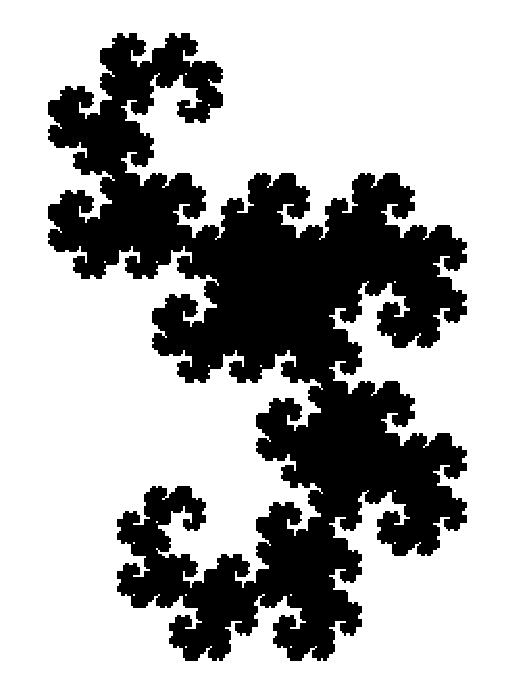
\includegraphics[height=7.5cm]{dragon.eps}

dragon $20$
\end{center}
\end{document}
